\documentclass{beamer}
\usepackage{graphicx}
\usepackage{amsmath, esint}

\usepackage{ragged2e}
\usepackage{tikz}
\usetikzlibrary{arrows,shapes}

\usepackage{listings}
\lstset{escapeinside={@(}{)@}}
\usepackage{algorithm}
\usepackage{algorithmic}

\usepackage{minted}
\usepackage{xcolor} 
\definecolor{LightGray}{gray}{0.975}

%\usetheme{Warsaw}
\usefonttheme{serif} 

\title[Chapter 4]{Database System Concepts, $7^{th}$ Edition \\ Chapter 4: Intermediate SQL}
\author{Silberschatz, Korth and Sudarshan}
\date{\today}

\setbeamertemplate{navigation symbols}{}%remove navigation symbols

\defbeamertemplate*{footline}{shadow theme}
{%
  \leavevmode%
  \hbox{\begin{beamercolorbox}[wd=.5\paperwidth,ht=2.5ex,dp=1.125ex,leftskip=.3cm plus1fil,rightskip=.3cm]{author in head/foot}%
    \usebeamerfont{author in head/foot} Database System Concepts \hfill \insertshorttitle
  \end{beamercolorbox}%
  \begin{beamercolorbox}[wd=.5\paperwidth,ht=2.5ex,dp=1.125ex,leftskip=.3cm,rightskip=.3cm plus1fil]{title in head/foot}%
    \usebeamerfont{title in head/foot} \hfill \insertframenumber\,/\,\inserttotalframenumber%
  \end{beamercolorbox}}%
  \vskip0pt%
}

\AtBeginSection[]
{
     \begin{frame}<beamer>
     \frametitle{Plan}
     \tableofcontents[currentsection]
     \end{frame}
}

\newcommand{\toRight}[1]{
    \begin{FlushRight}
        {\tiny #1}
    \end{FlushRight}
} % Align to right

\begin{document}

\frame{\titlepage}

\begin{frame}{Database System Concepts}
    \centering
    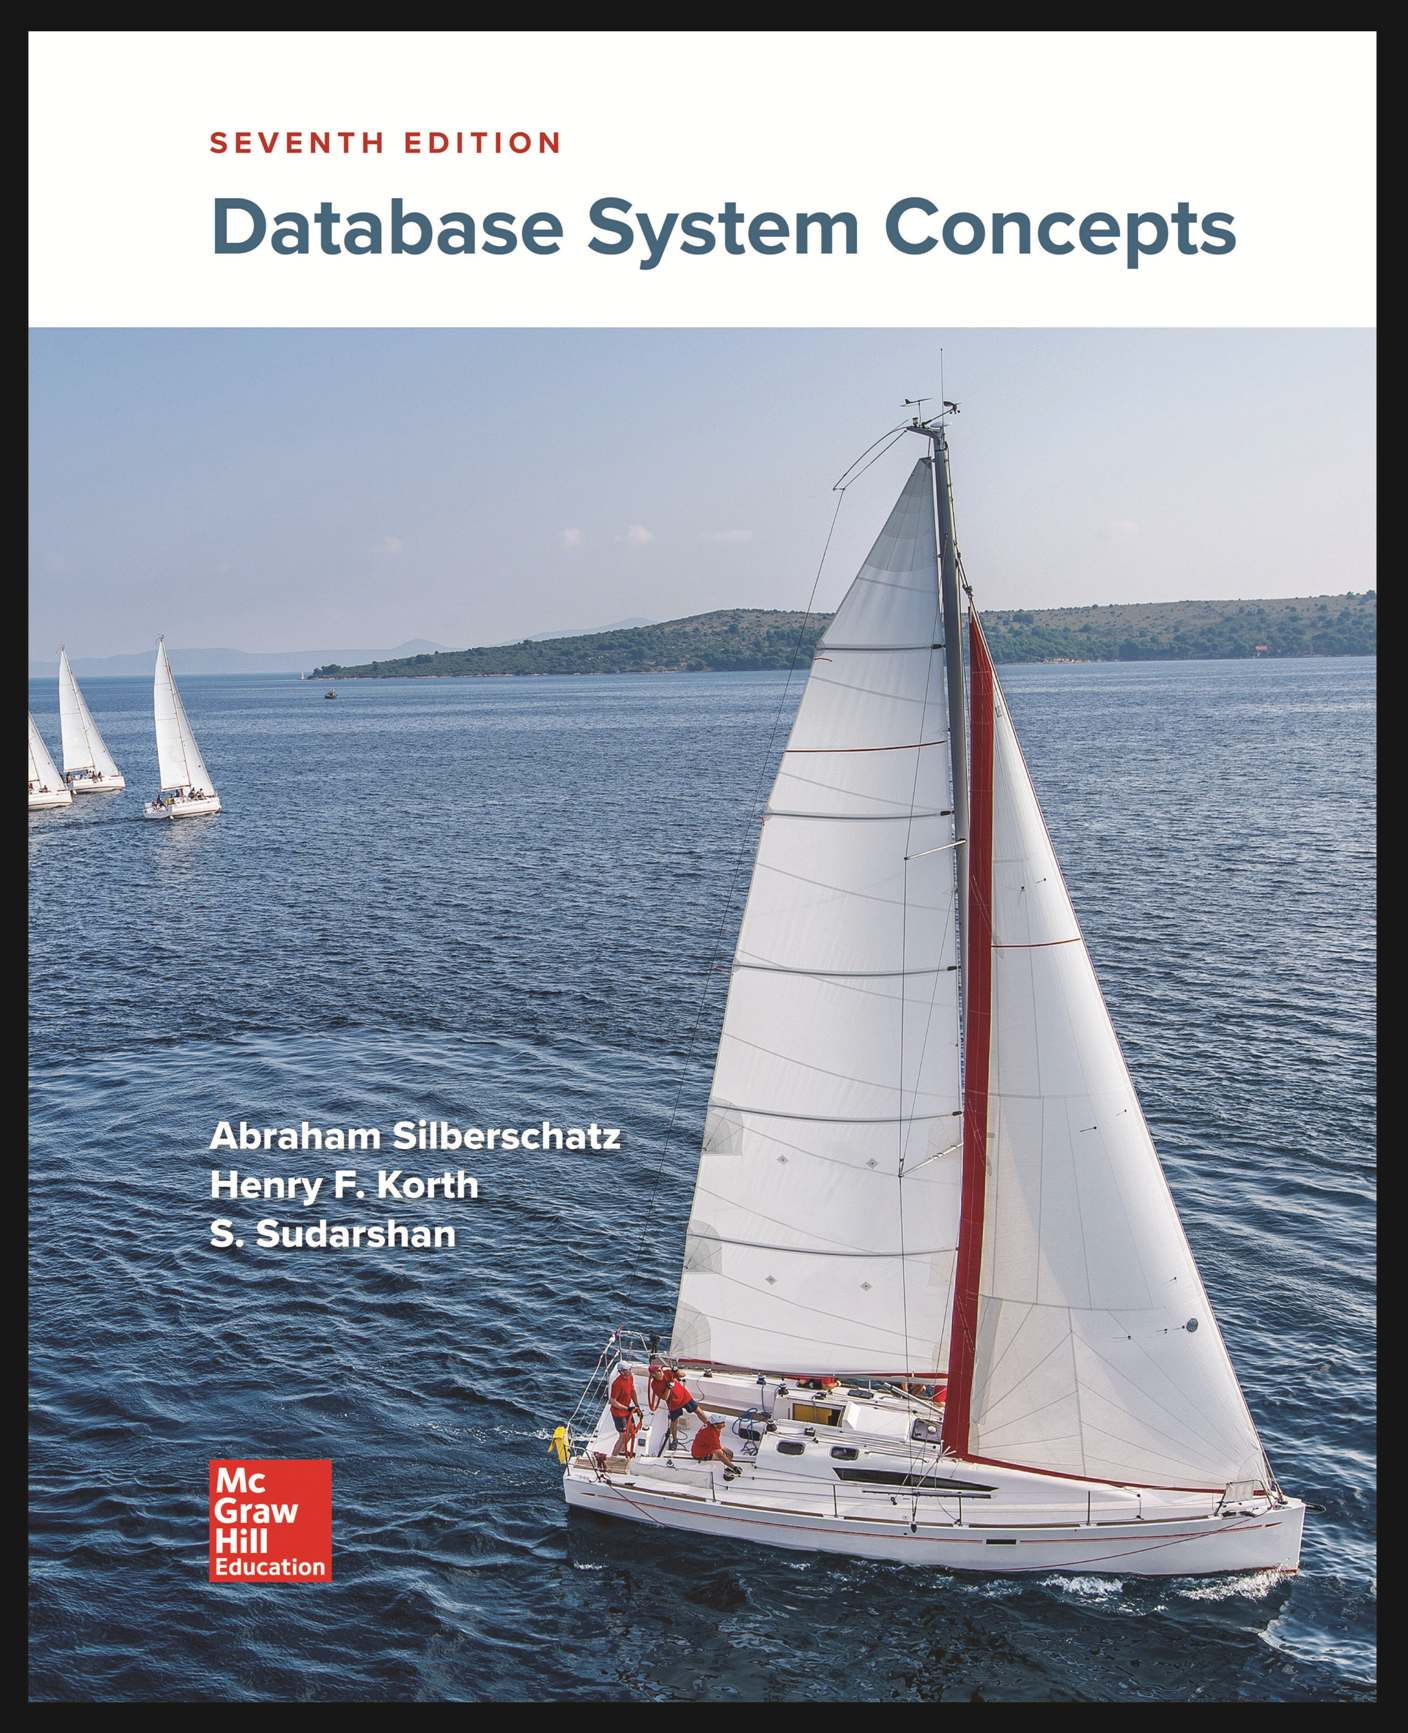
\includegraphics[width=0.5\textwidth]{figures/book_cover.jpg} \\
    \vspace{5mm}
    {
        \tiny
        Content has been extracted from \textit{Database System Concepts}, Seventh Edition, by Silberschatz, Korth and Sudarshan. Mc Graw Hill Education. 2019.\\
        Visit \url{https://db-book.com/}.\\
    }
\end{frame}

\section{Join Expressions}

\begin{frame}{Joined Relations}
    \begin{itemize}
        \item Join operations take two relations and return as a result another relation.
        \item A join operation is a Cartesian product which requires that tuples in the two relations match (under some condition). It also specifies the attributes that are present in the result of the join.
        \item The join operations are typically used as subquery expressions in the from clause.
        \item Three types of joins:
        \begin{itemize}
            \item Natural join
            \item Inner join
            \item Outer join
        \end{itemize}
    \end{itemize}
\end{frame}

\begin{frame}[fragile]{Natural Join in SQL}
    \begin{itemize}
        \item Natural join matches tuples with the same values for all common attributes, and retains only one copy of each common column.
        \item List the names of instructors along with the course ID of the courses that they taught.
        \begin{minted}
        [tabsize=4, obeytabs, frame=lines, framesep=2mm, baselinestretch=1.2, bgcolor=LightGray, fontsize=\footnotesize, linenos]{sql}
        SELECT
            name, course_id
        FROM
            students, takes
        WHERE
            student.ID = takes.ID;
        \end{minted}
    \end{itemize}
\end{frame}

\begin{frame}[fragile]{Natural Join in SQL}
    \begin{itemize}
        \item Same query in SQL with ``natural join'' construct.
        \begin{minted}
        [tabsize=4, obeytabs, frame=lines, framesep=2mm, baselinestretch=1.2, bgcolor=LightGray, fontsize=\footnotesize, linenos]{sql}
SELECT
    name, course_id
FROM
    student NATURAL JOIN takes;
        \end{minted}
    \end{itemize}
\end{frame}

\begin{frame}[fragile]{Natural Join in SQL (Cont.)}
    \begin{itemize}
        \item The \texttt{FROM} clause in can have multiple relations combined using natural join:
        \begin{lstlisting}[language=SQL]
SELECT @($A_1, A_2, \ldots, A_n$)@
FROM @($r_1$)@ 
    NATURAL JOIN @($r_2$)@ 
    NATURAL JOIN @($\ldots$)@ 
    NATURAL JOIN @($r_n$)@
WHERE @($P$)@;
        \end{lstlisting}
    \end{itemize}
\end{frame}

\begin{frame}{Student Relation}
    \centering
    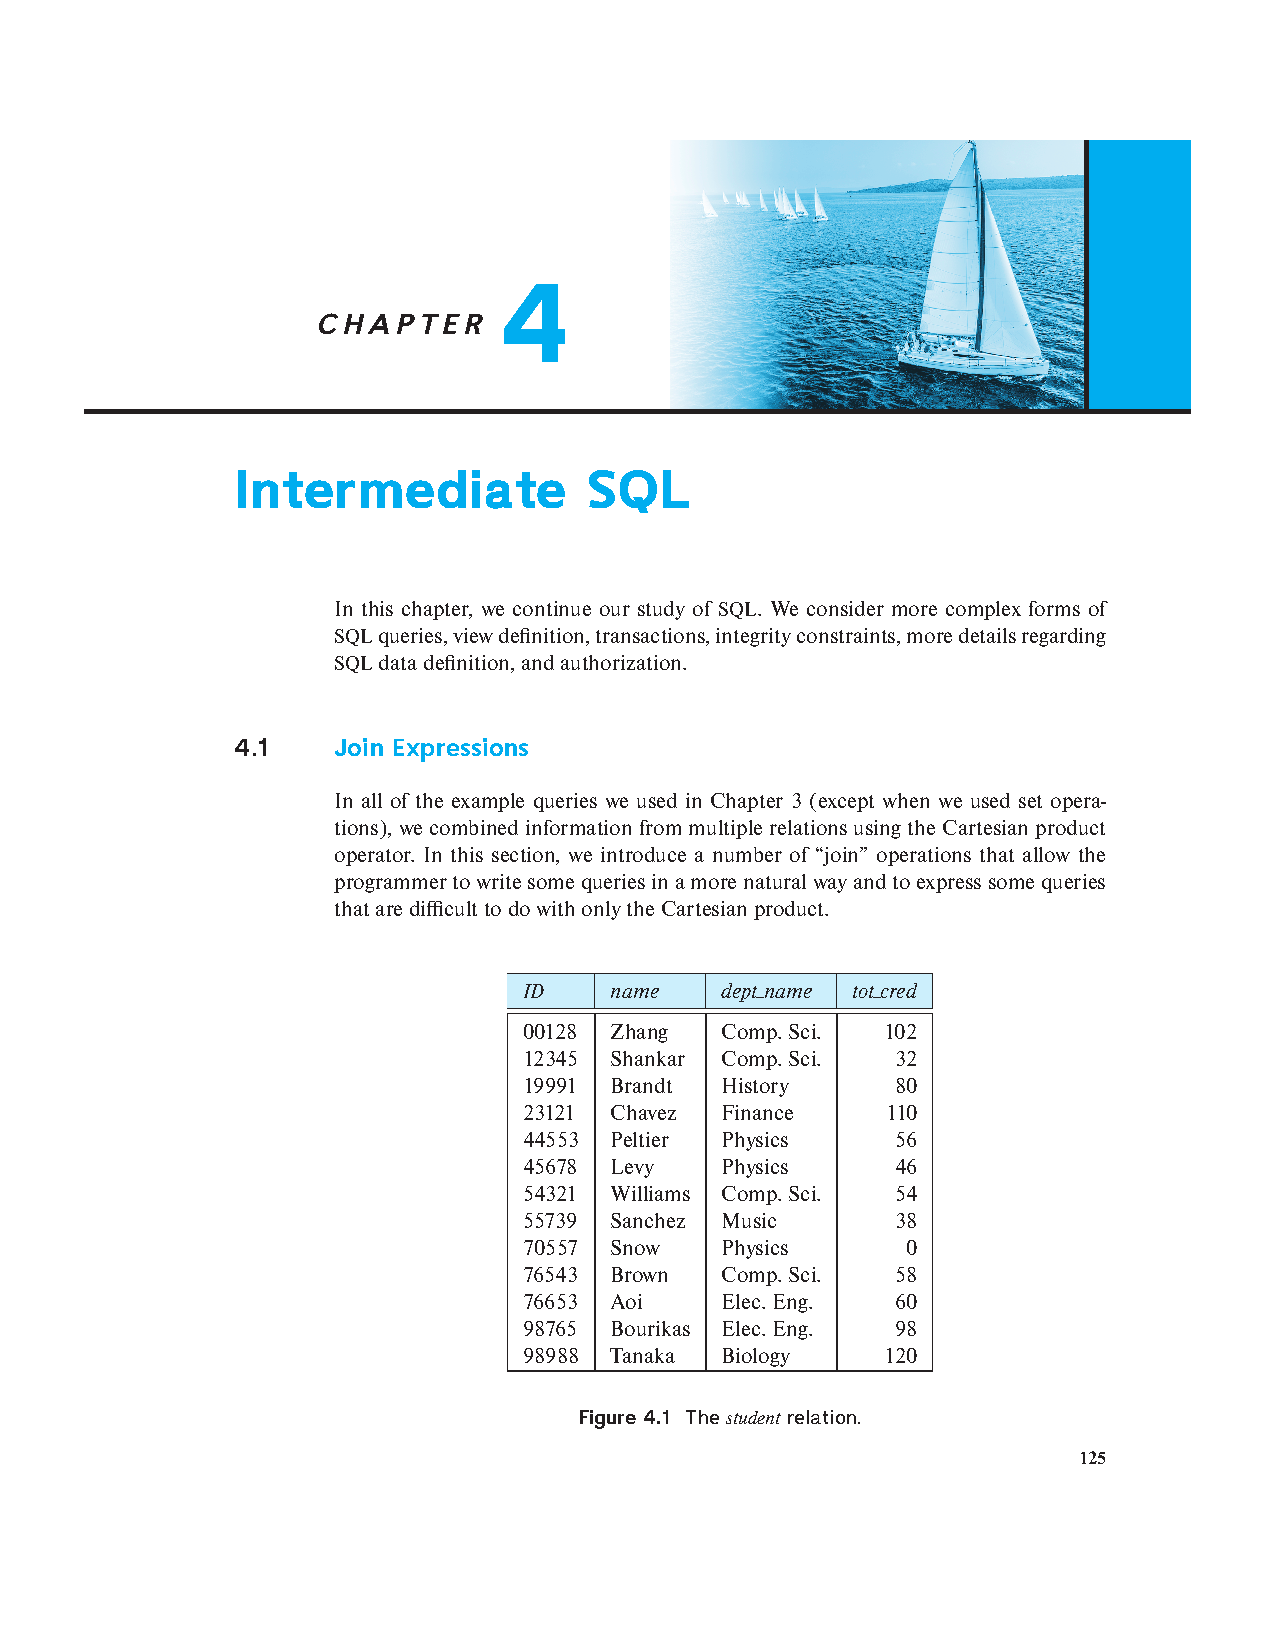
\includegraphics[width=0.75\textwidth, trim={8cm 4.5cm 5cm 16cm}, clip]{pages/nj1.pdf}
\end{frame}

\begin{frame}{Takes Relation}
    \centering
    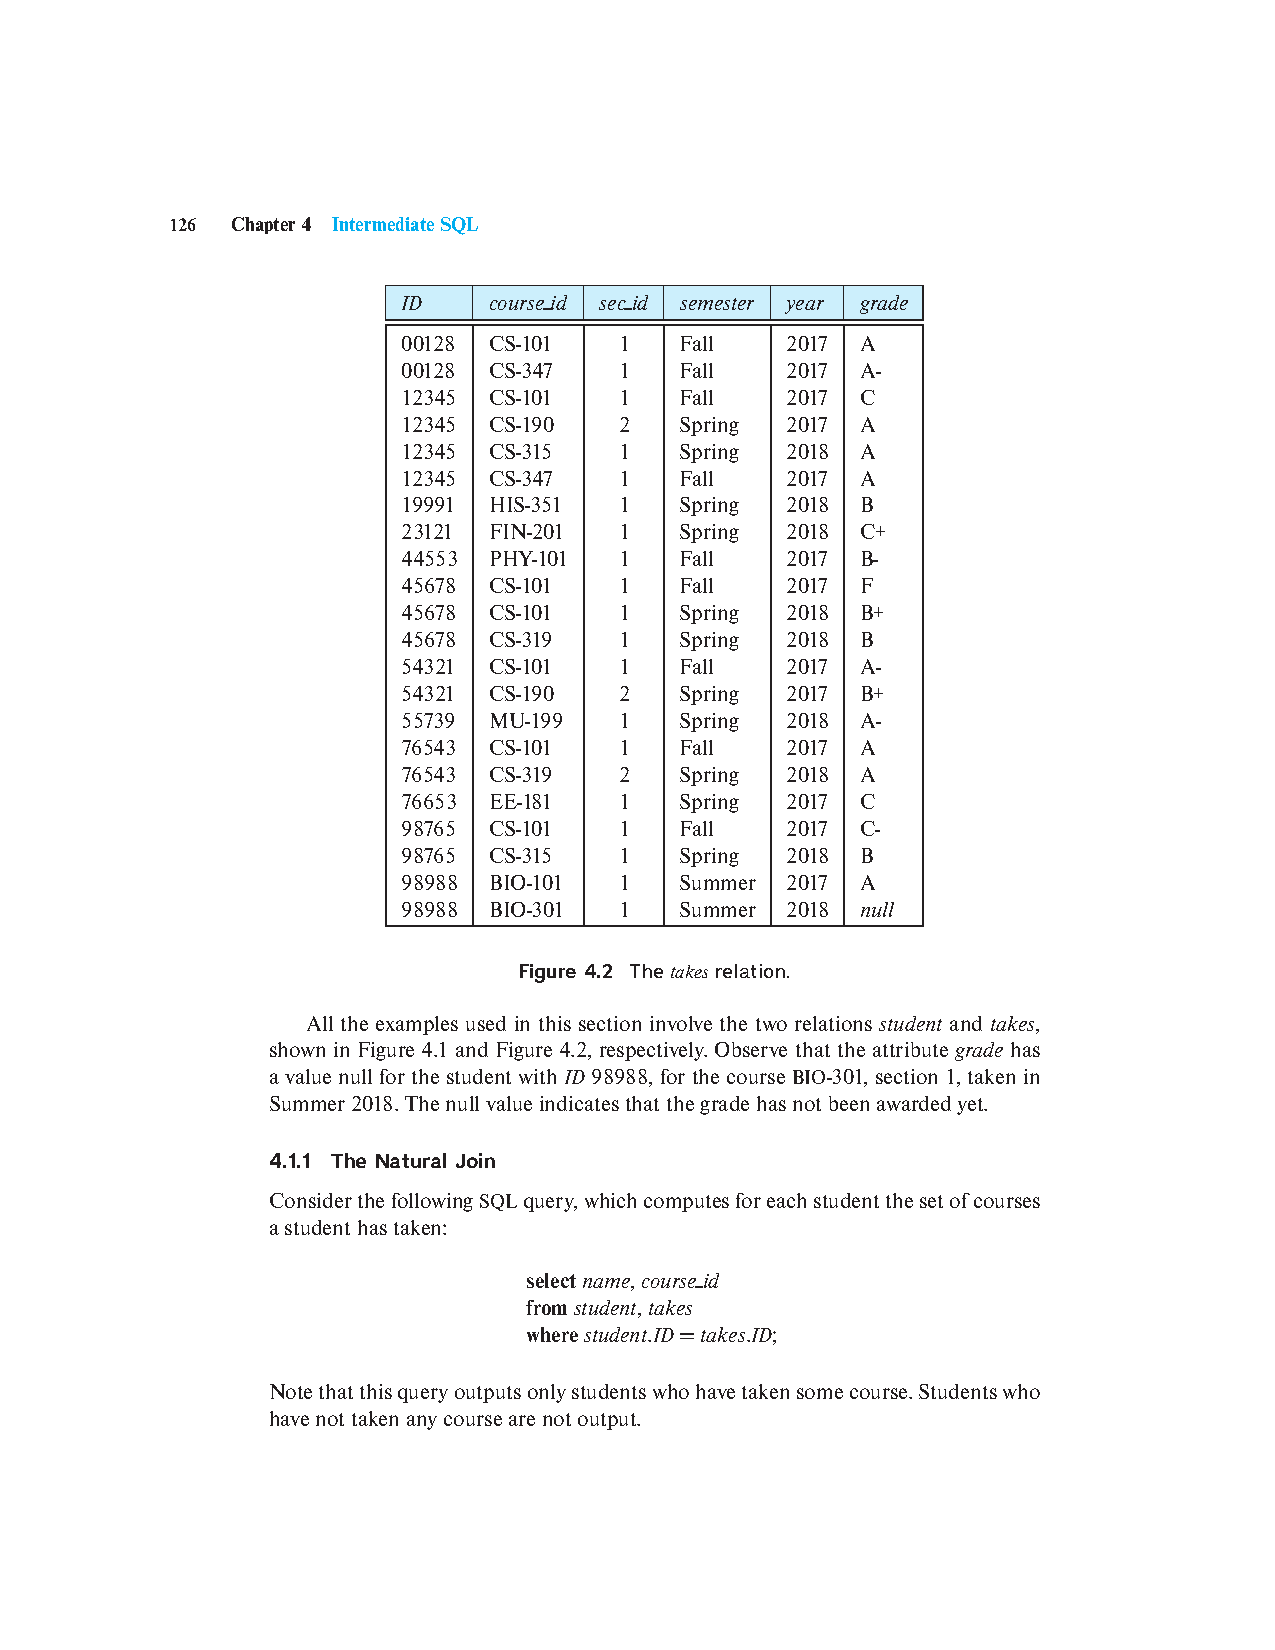
\includegraphics[width=0.75\textwidth, trim={4.5cm 12cm 5.5cm 4.5cm}, clip]{pages/nj2.pdf}
\end{frame}

\begin{frame}{Student Natural Join Takes}
    \centering
    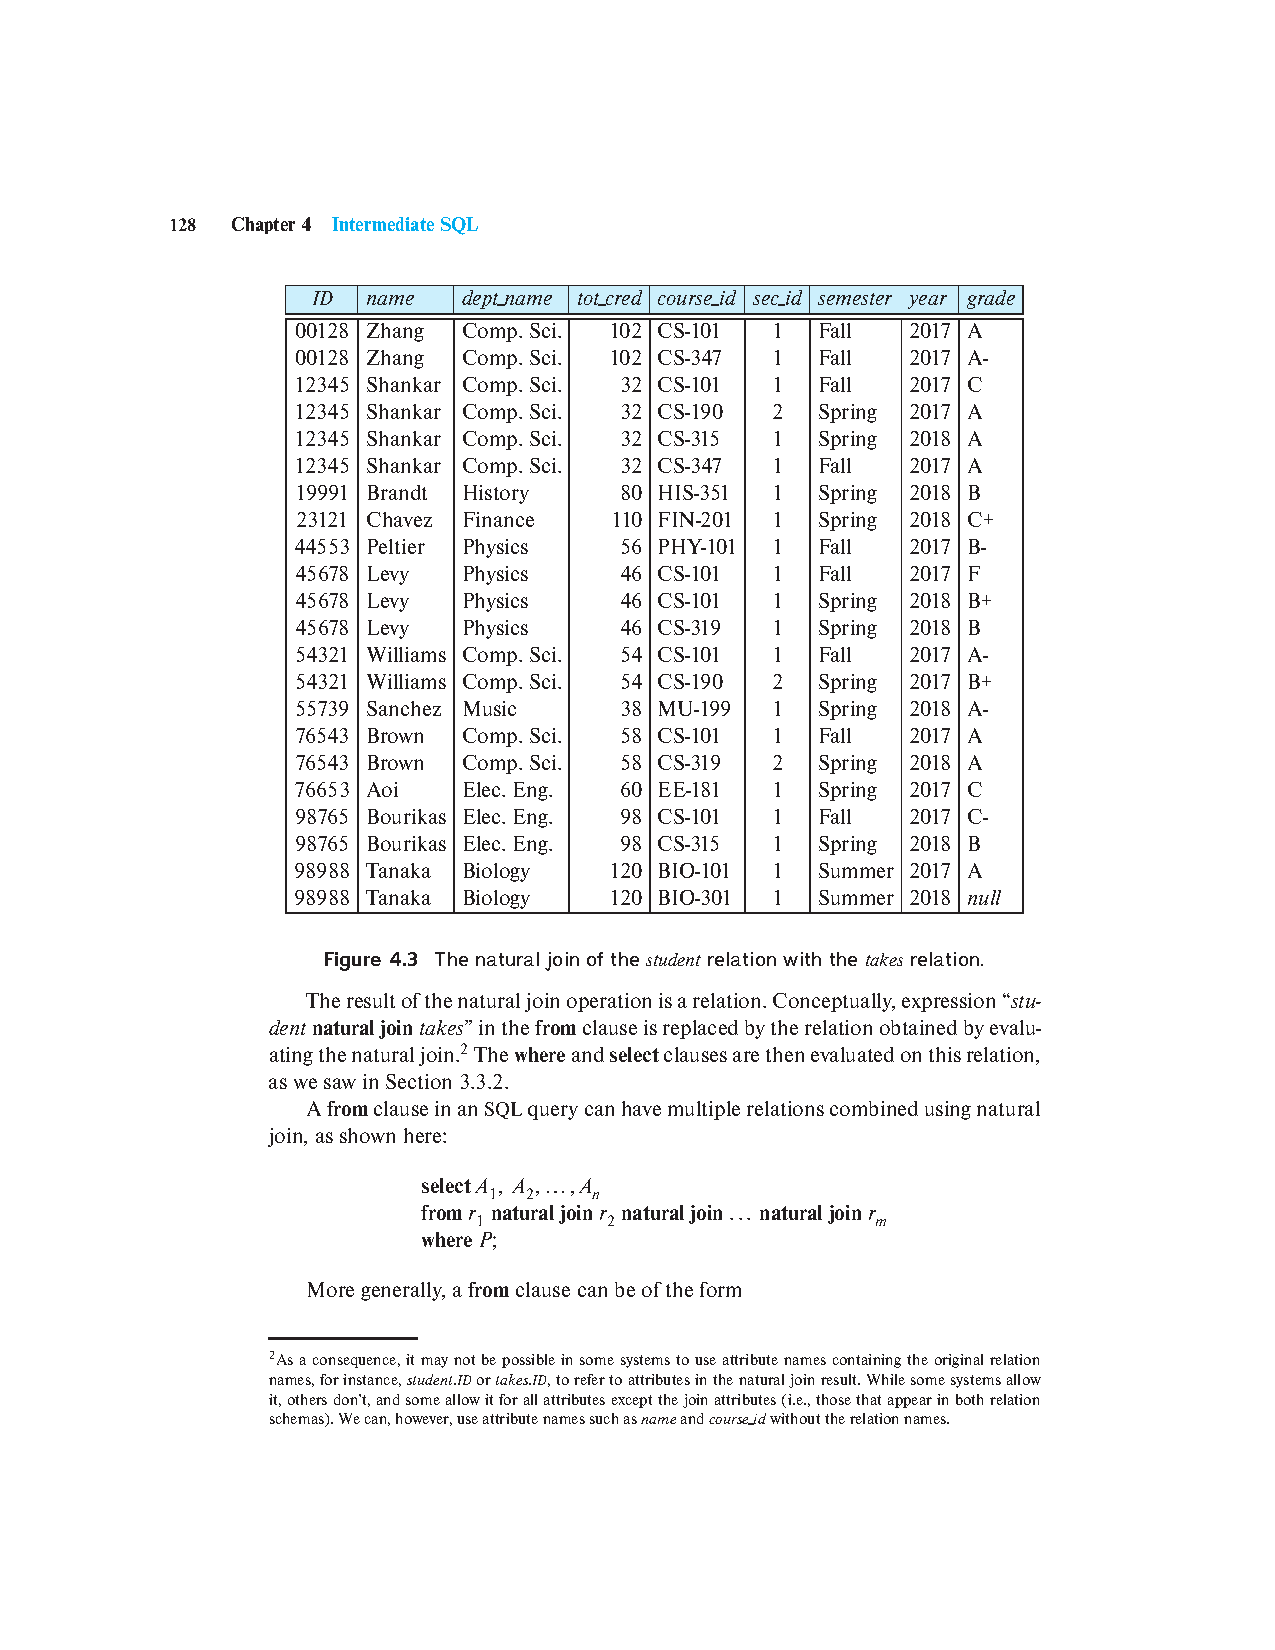
\includegraphics[width=0.95\textwidth, trim={3cm 12cm 3cm 4.5cm}, clip]{pages/nj3.pdf}
\end{frame}




\section{Views}
\section{Transactions}
\section{Integrity Constraints}
\section{SQL Data Types and Schemas}
\section{Index Definition in SQL}
\section{Authorization}

\begin{frame}[fragile]{}
    \begin{minted}
    [tabsize=4, obeytabs, frame=lines, framesep=2mm, baselinestretch=1.2, bgcolor=LightGray, fontsize=\footnotesize, linenos]{sql}
    \end{minted}
\end{frame}

\begin{frame}{}
\end{frame}

% \begin{frame}{}
%      \centering
%      \Huge End of Chapter 4.
% \end{frame}

% \section*{Takeaways}
% 
% % Tim Duncan's Top 5 Fundamental Takeaways of the Today's Class
% \begin{frame}{TDT5FTOTTC}
%     \centering
%     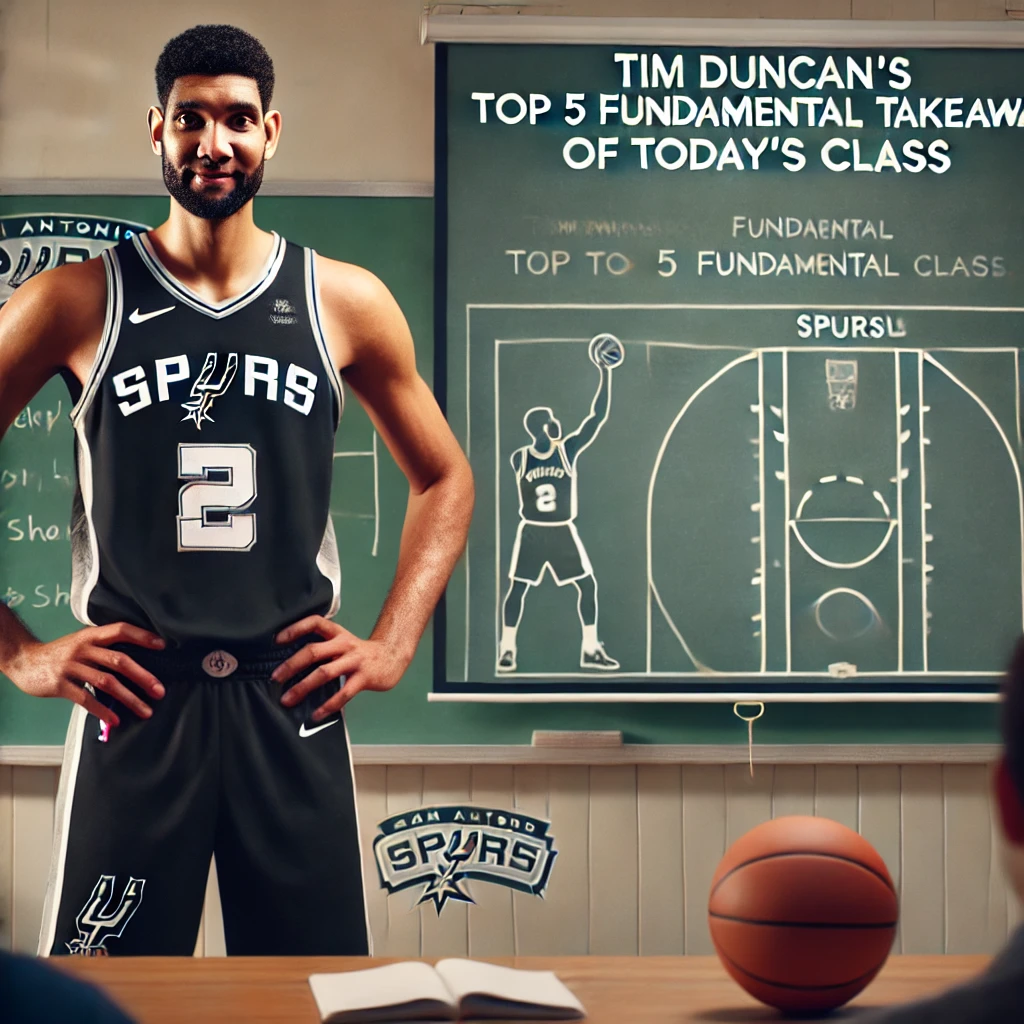
\includegraphics[width=0.75\textwidth]{figures/tim.png}
% \end{frame}
% 
% \begin{frame}{Top 5 Fundamental Takeaways}
%     \small
%     \begin{enumerate} \pause
%         \item[5] \textbf{}. \pause
%         \item[4] \textbf{}. \pause
%         \item[3] \textbf{}. \pause
%         \item[2] \textbf{}. \pause
%         \item[1] \textbf{}.
%     \end{enumerate}
% \end{frame}

\begin{frame}{Database System Concepts}
    \centering
    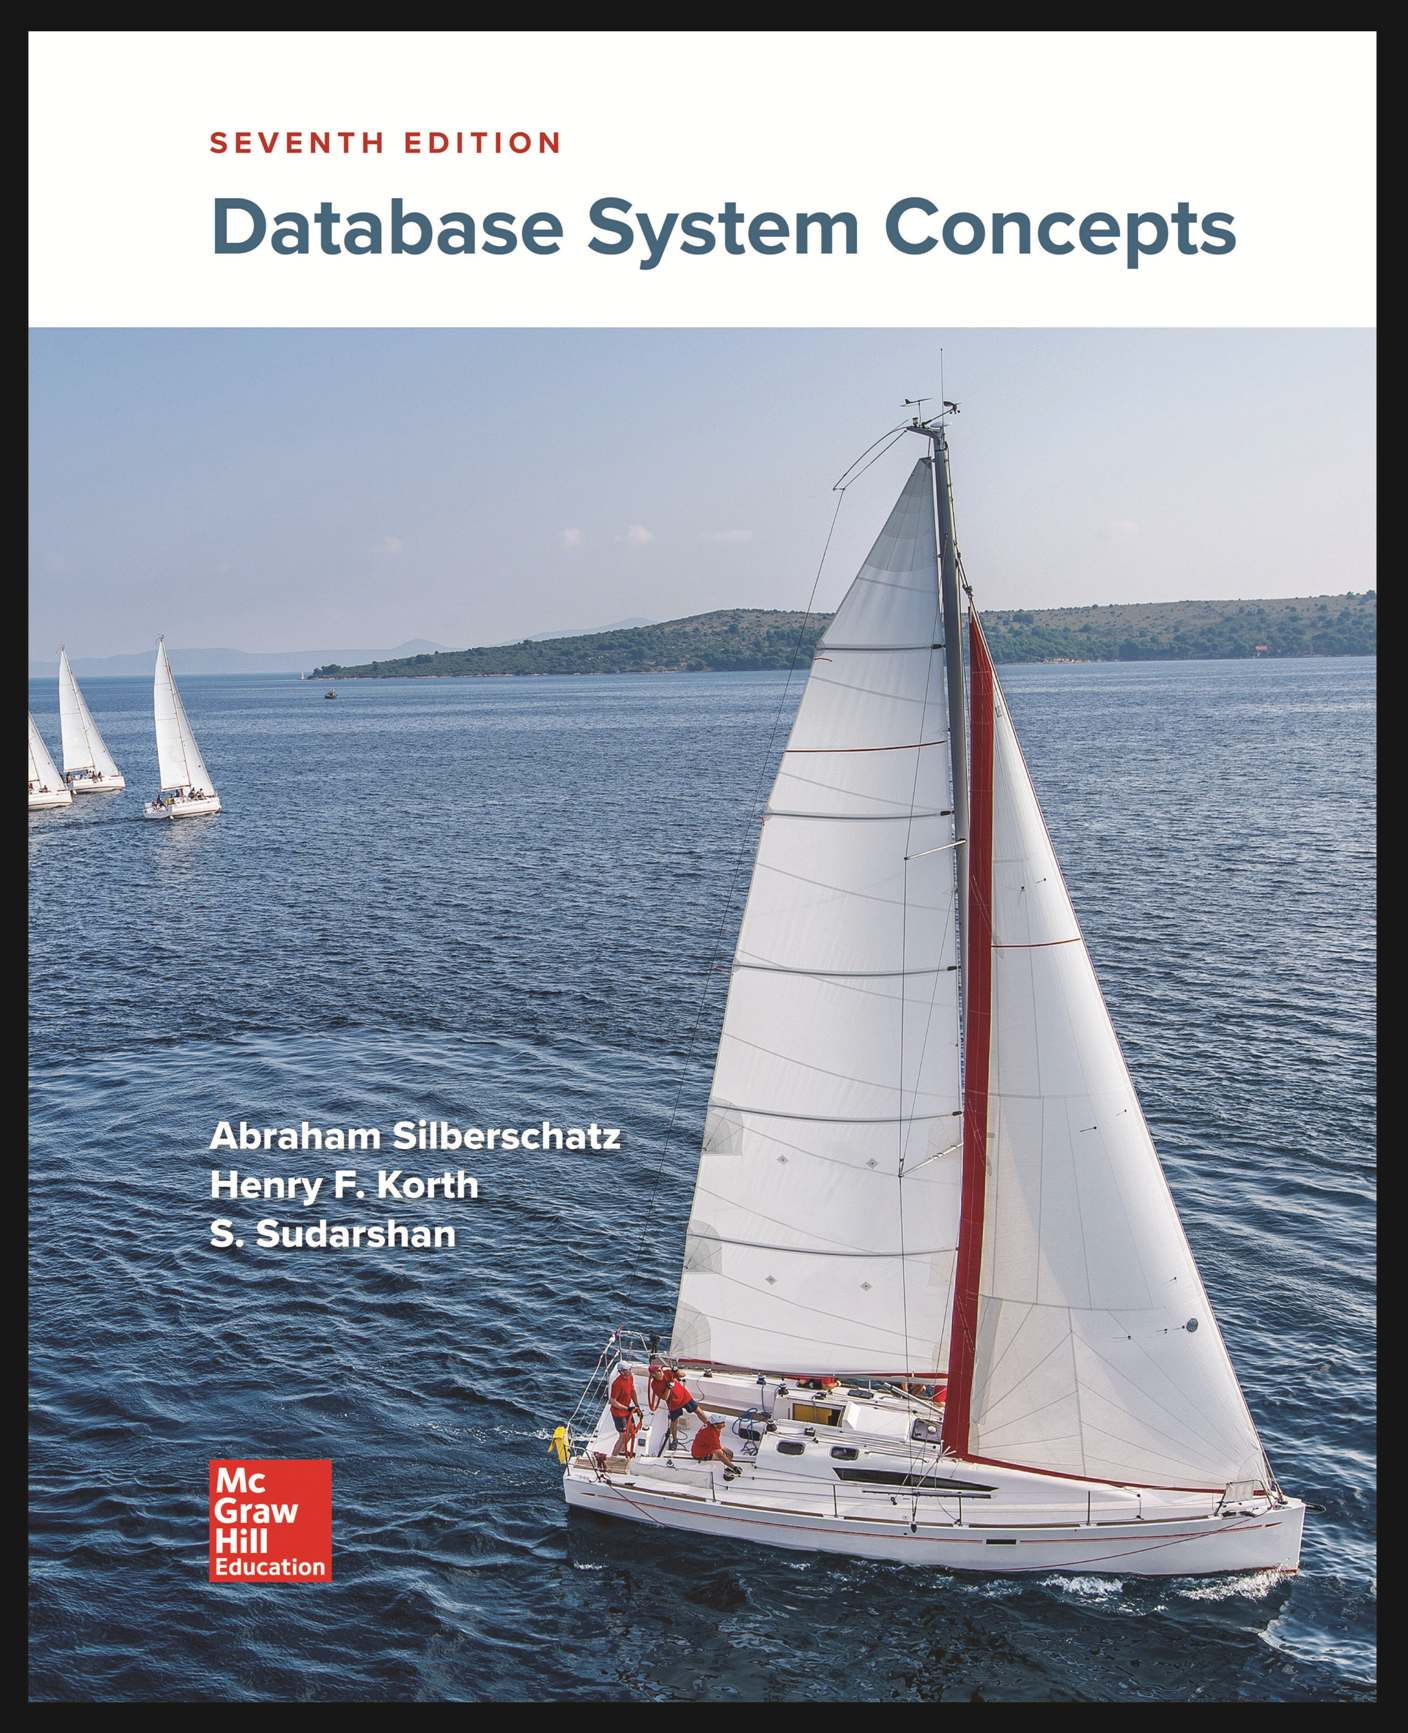
\includegraphics[width=0.5\textwidth]{figures/book_cover.jpg} \\
    \vspace{5mm}
    {
        \tiny
        Content has been extracted from \textit{Database System Concepts}, Seventh Edition, by Silberschatz, Korth and Sudarshan. Mc Graw Hill Education. 2019.\\
        Visit \url{https://db-book.com/}.\\
    }
\end{frame}

\end{document}
